\documentclass[12pt,a4paper]{article}

\usepackage{graphicx}
\usepackage{abstract}
\usepackage{hyperref}
\usepackage{listings}
\usepackage{indentfirst}

\graphicspath{ {./images/} }
\renewcommand{\abstractname}{\large{Timestamps}}

\setlength{\parindent}{0.5in}

\title{CPSC 361 | Homework \#1 \\(Including Project Details)}
\author{Chris Nutter\thanks{Dedicated to @QuesoGrande a.k.a. Jared D.}}

% --> Here we go, satellite radio, y'all get hit with a...

\begin{document}

\maketitle

\begin{abstract}
    \noindent
    \begin{center}\textbf{09/09/2020 - 09:36:10 AM}\end{center}
    You may want to skip the first section because it is for our group project and does not involve the textbook or python code.\\
    \begin{center}\textbf{09/12/2020 - 12:58:05 PM}\end{center}
    Sorry if there is weird spacing with the timestamps. I am currently working on fixing this. This timestamp will be deprecated if I fix the issue.\\
\end{abstract}

\tableofcontents    

% -->

\section{How the Project Will Work?}
    The application will be a very simple interface dedicated towards children to make sure they can follow along easily while retaining the information. Simple math is the goal while also expanding their mathematical knowledge. It'll be fairly straightforward. Multiple choice will be the way to go because it has proven to help decipher knowledge for students in the educational field. We will have a point system to tally up points per student. The more points they have, the better they're doing. The lower the points, the worse they are doing. If a student has 0 points, they are about the level we expect them to be at and we hope for them to be higher overtime. If they are lower than 0, they express issues with the topics at hand. Each problem will also have a time limit and a skip button. The time limit is set so the students don't use calculators and they work on their own. The skip button is there to provide a way to come back to the problem. Each session has a set time limit where all problems will be finished which challenges the student's to work diligently.\par
    \begin{center}\line(1,0){250}\end{center}

% -->

\section{Chapter 1 Summary}
In the opening statements, we have a conversation between a software engineer and a game developer. The developer explains that they need to adapt a software engineering mindset towards their games or else they cannot make it out of the field alive. The textbook later explains that since technology is ever expanding, software is very important and that it requires pretty much most engineering products need some sort of software to be able to run. Software today is considered a product and just like packaging meat for a deli, we are creating a product for customers to use and it is very important for us as developers and engineers to make sure the software we deliver follow the guidelines for the industry. Unlike the early days of software engineering, we in the 21st century develop code that is proper and respectable and maintain a level of efficiency and help towards a company.\par
    The industry has changed dramatically over the years due to many improvements in hardware (as well as software). Even with major advancements, we are still getting the reverberations of scrutiny towards programmers. The nature of software is ever-changing. It changes fairly often because of how technology advances everyday.\par
    WebApps are becoming more and more common because new websites pop up everyday. Before, WebApps were mostly linked hypertext that were very limited. Now it has evolved into a huge set of languages and projects. Many main PC applications are now fully on web without needing desktop clients. This does come with its disadvantages like databases being unreliable security-wise and easy access to intrusions just when loading a website alone. Mobile applications also have improved dramatically over the years. Each application is designed with a small portable screen at hand which is why you rarely see desktop apps ported to mobile (you usually seem them rewritten from the ground up). Cloud computing is now one of the biggest ecosystems in the software engineering space mainly due to its cheaper finance for the end user and its more control over the end user. While cloud computing is useful for many as it does not rely heavily on the end-user, it gives companies more control over the software/information at hand creating a blockage between what information the company is obtaining or not. Cloud computing is the upcoming future for our children whether people want it or not.\par
    Product Line Software is defined as 'a set of software-intensive systems that share a common, managed set of features satisfying the specific needs of a particular market segment or mission and that are developed from a common set of core assets in a prescribed way." [SEI13]. This concept is very important to software engineers because it helps maintain a set of particular needs from both the front-end and back-end of a project. It helps maintain a sense of balance between the two main fields.\par 
    The main issue with software engineers is time and demand. Are we able to create a project within the deadline to the specifications? Are concepts going to be cut? Who is in charge of the cutting process the people that can code or the people who want you to code? This is the ethical dilemma that mostly all software engineers face in their lifetime and there is no clear ways to solve this problem.
    \begin{center}\line(1,0){250}\end{center}

% -->

\section{Python Test Code \& Output}
   \begin{center}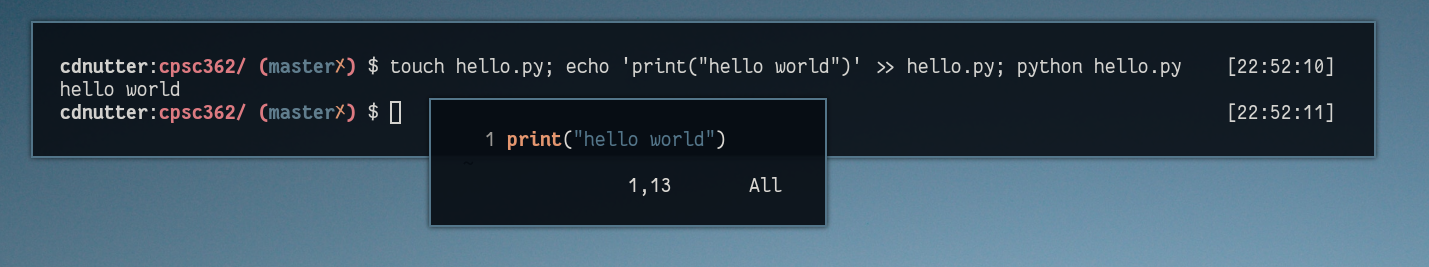
\includegraphics[width=13.8cm]{python-test.png}\end{center}
    I created a python project that outputs hello world with one line in Terminal. 
    It creates a
    \begin{lstlisting}[language=bash]
        $ hello.py
    \end{lstlisting}
    which inputs
    \begin{lstlisting}[language=Python] 
        $ print('hello world') 
    \end{lstlisting} inserts the code, and executes the script. Since python's hello world is a one-liner. I needed to do something to make it a little cooler. 
\end{document} 
